% Setup
\documentclass[12pt]{article}

% Packages
\usepackage{geometry}
\usepackage{color}
\usepackage{lingmacros}
\usepackage{amsmath}
\usepackage{siunitx}
\usepackage{graphicx}
\usepackage[svgnames]{xcolor}
\usepackage{listings}
\usepackage{csquotes}
\usepackage{float}
\usepackage[italicdiff]{physics}
\usepackage{url}
\usepackage{titling}

% Setup title
\setlength{\droptitle}{-80pt}
\posttitle{\par\end{center}} % Removes spacing between properties
\preauthor{}  % Remove the spacing added by
\postauthor{} % the author property.
\title{PSBC Project 3: Purchasing Data Analysis}
\date{\today}
\author{} % No author

% Slightly bigger size: \scriptsize
\lstset{
  language=Matlab,                     % the language of the code
  basicstyle=\scriptsize\ttfamily, % the size of the fonts that are used for the code
  numbers=left,                   % where to put the line-numbers
  numberstyle=\scriptsize\color{Blue},  % the style that is used for the line-numbers
  stepnumber=1,                   % the step between two line-numbers. If it is 1, each line
                                  % will be numbered
  numbersep=5pt,                  % how far the line-numbers are from the code
  backgroundcolor=\color{white},  % choose the background color. You must add \usepackage{color}
  showspaces=false,               % show spaces adding particular underscores
  showstringspaces=false,         % underline spaces within strings
  showtabs=false,                 % show tabs within strings adding particular underscores
  frame=single,                   % adds a frame around the code
  rulecolor=\color{black},        % if not set, the frame-color may be changed on line-breaks within not-black text (e.g. commens (green here))
  tabsize=2,                      % sets default tabsize to 2 spaces
  captionpos=t,                   % sets the caption-position to bottom
  breaklines=true,                % sets automatic line breaking
  breakatwhitespace=false,        % sets if automatic breaks should only happen at whitespace
  deletekeywords={data,frame,length,as,character},
  keywordstyle=\color{RoyalBlue},      % keyword style
  otherkeywords={},
  commentstyle=\color{DarkGreen},   % comment style
  stringstyle=\color{ForestGreen}      % string literal style
}

\lstset{literate=%
   *{0}{{{\color{RoyalBlue}0}}}1
    {1}{{{\color{RoyalBlue}1}}}1
    {2}{{{\color{RoyalBlue}2}}}1
    {3}{{{\color{RoyalBlue}3}}}1
    {4}{{{\color{RoyalBlue}4}}}1
    {5}{{{\color{RoyalBlue}5}}}1
    {6}{{{\color{RoyalBlue}6}}}1
    {7}{{{\color{RoyalBlue}7}}}1
    {8}{{{\color{RoyalBlue}8}}}1
    {9}{{{\color{RoyalBlue}9}}}1
    {TRUE}{{{\color{RoyalBlue}TRUE}}}4
    {FALSE}{{{\color{RoyalBlue}FALSE}}}5
    {<-}{{{\color{Gray}<-}}}2
}

% Commands/Setup
%%%%%%%%%%%%%%%%%%%%%%%%%%%%%%%%%%%%%%%%%%%%%%%%%%%%%%%%%%%%%%%%%%%%%%%%%%%%%%%%%%%%%
\newcommand{\vect}[1]{\underline{\boldsymbol{#1}}}
\newcommand{\mat}[1]{\underline{\underline{\boldsymbol{#1}}}}
\newcommand{\mean}[1]{\bar{#1}}
\newcommand{\trans}[1]{#1^T}
\newcommand{\est}[1]{\hat{#1}}
\newcommand{\bfrac}[2]{\left(\frac{#1}{#2}\right)}
\newcommand{\bb}[1]{\left(#1\right)}
\newcommand{\inprod}[2]{\langle#1\,#2\rangle}
\renewcommand{\exp}[1]{\text{exp}\left(#1\right)}
\newcommand{\e}[1]{\text{e}^{#1}}
\newcommand{\hl}[1]{``\path{#1}"}

% Note: this solution isn't compatible with hyperref package
\let\oldref\ref
\renewcommand{\ref}[1]{(\oldref{#1})}
\newcommand{\apref}[1]{App-\ref{#1}}
\newcommand{\figref}[1]{Fig-\ref{#1}}
%%%%%%%%%%%%%%%%%%%%%%%%%%%%%%%%%%%%%%%%%%%%%%%%%%%%%%%%%%%%%%%%%%%%%%%%%%%%%%%%%%%%%%

% Setup each page
\geometry{
a4paper,
left=15mm,
top=17mm,
bottom=17mm,
right=15mm,
heightrounded
}
\setlength{\parindent}{0em}
\setlength{\parskip}{1em}

\graphicspath{{./Images/}}

% Document
\begin{document}

% Title page
\maketitle

\section*{Introduction}
Note that any reference with prefix ``App-", refers to a piece of code listing given in the appendix. An example of this is App-(1).

% Start
\section{Question 1}
For this question, we want to find a probability logistic function that a product is returned when given the rating $r$ for a customer. The function can be given with the two constant parameters $\alpha$ and $\beta$ as:
\begin{equation*}
  P(r) = \frac{1}{1+\exp{-\alpha r - \beta}}
\end{equation*}
Hence for this question, we want to find the values of $\alpha$ and $\beta$ which minimise the difference between the estimated probability function and the actual probability.

\subsection{Reading and filtering the data}
We first start of with reading the data from the \hl{purchasing_order.csv} file directly into a Matlab table using the \hl{readtable} function, passing in the file name as a parameter. After we have read the file, we want to remove all rows from the table which have a rating of zero. The reason we do this is because a rating of zero implies that the purchase has not been rated, hence we cannot associate if it was the customers opinion on the product which was the reason for whether the customer has or has not returned it. We can do this with the following code:
\begin{lstlisting}[title={Reading and filtering the data}]
% Read file and format into table.
dataTable = readtable('purchasing_order.csv');
% Filter out data where rating is 0.
dataTable(dataTable.Rating == 0, :) = [];
\end{lstlisting}
After we have the filtered table, we want to get the two arrays we wish to work with, the \hl{Rating} and \hl{Return} columns. To get the ratings we just use the function \hl{table2array}, and pass in the \hl{Rating} column from \hl{dataTable}, which converts the table column to an array. However, for the \hl{Return} column, we have the data in terms of `Y' and `N'. Obviously for data analysis, we do not want it in this form, instead we want it as one's or zero's. Hence after we get the array, we can just compare it equivalently against ``Y". The code for this is given as:
\begin{lstlisting}[title={Getting the two arrays}]
% Get 2 arrays from the table columns of Rating and Return.
% We just pass in the Rating column from dataTable.
Rating = table2array(dataTable(:, 'Rating'));
% Note we want our array in terms of Pass (1) or fail (0), not 'Y' or 'N',
% so we do a simply boolean equality check against 'Y' for each element in
% the column. We check against the string "Y", as table2array returns an
% array of cells.
Return = table2array(dataTable(:, 'Return')) == "Y";
\end{lstlisting}

\subsection{Finding the parameters}
To find the ideal parameters, we will be using the method of minimising the error. To do so we first create an anonymous function which returns the sum of the entries of the vector difference between some true valued vector, and the probability logarithmic function vector. We then use the \hl{fminsearch} function, where we pass in our anonymous function with inputs of the Rating and Return vectors, and an initial point of the parameters as $\alpha=0, \beta=0$. \hl{fminsearch} will then find the values of the parameters which minimise the anonymous function (which is the error). The code for this is given as:
\begin{lstlisting}[title={Finding the parameters}]
% Create a short function, which gets the sum of the entries, of the
% difference between the true value of the Return (p) and the logarithmic
% function, for the logarithmic parameters (a), and the Rating input (h).
logreg = @(a,h,p) sum((p-(1+exp(-a(1)*h-a(2))).^(-1)).^2);

% Find the parameters (a) which minimise the sum difference of logreg,
% given the data of Rating and Return.
a = fminsearch(@(a) logreg(a,Rating,Return),[0 0]);  % Output: -15.4074   13.7003
a % Print the value.
\end{lstlisting}
This gives our output as:
\begin{lstlisting}[title={Finding the parameters}]
a =
  -15.4074   13.7003
\end{lstlisting}
That is, we get $\alpha=-15.4074$, and $\beta=13.7003$.

\subsection{Validating the parameters}
We want to know whether the parameters we found seem statistically correct. To do so we can look at the values we get for each rating, and compare them to the data from the table. We first start by creating a vector with entries from one to five, representing the valid ratings. Then we simply pass this into the probability logarithmic function. The code for this is:
\begin{lstlisting}[title={Checking the parameters}]
% Create vector of 1 to 5 integers.
x = linspace(1, 5, 5)
% Create vector using regression function with found parameters, and pass
% in ratings from x.
y = (1+exp(-(x*a(1)+a(2)))).^-1
\end{lstlisting}
From this we get our result as:
\begin{lstlisting}[caption={Checking the parameters}, label={1_test}]
x =
     1     2     3     4     5
y =
    0.1535    0.0000    0.0000    0.0000    0.0000
\end{lstlisting}
So now we can do two simply checks; first, how many returns have we had with a rating equal of greater than two; second, what is the percentage of the amount of returns with a rating of one against the total amount of returns. We can check this with the following:
\begin{lstlisting}[title={Checking the parameters}]
% Print the number of rows where the Rating column is greater than or equal
% to 2, and has a return.
height(dataTable((dataTable.Rating >= 2) & (dataTable.Return == "Y"), :))
% Get the subtable from dataTable with a rating of 1.
oneRating = dataTable(dataTable.Rating == 1, :);
% Print the percentage of those who returned the product against all the
% purchases from the oneRating table.
height(oneRating(oneRating.Return == "Y", :))/height(oneRating)
\end{lstlisting}
Which gives the result as:
\begin{lstlisting}[title={Result from checking the parameters}]
ans =
     0
ans =
    0.1535
\end{lstlisting}
As we see, we have no returns with a rating of two or higher, which corresponds to the results in Listing  \ref{1_test}. Furthermore, the percentage of returns with a rating of one is equivalent to the result from Listing  \ref{1_test} for the rating one. Hence altogether this provides evidence that the parameters $\alpha=-15.4074$, and $\beta=13.7003$ provide the best fit for the probability logarithmic function.

The full code for this question is given in \apref{1_fullCode}.


\section{Question 2}
For this task we want to find out the likelihood that a customer will make future orders from the company if they have previously returned a product. We will calculate the likelihood for a single customer to return as the percentage of total value spent after the return over the total values of the four-year period, excluding any returned purchases. That is:
\begin{equation}
  \text{Likelihood} = \frac{\text{total value spent after return}}{\text{total value spent during four-year period}} \label{2_likelihood}
\end{equation}

\subsection{Finding the customers who have returned a product}
Similar to question 1, we start off by reading the \hl{purchasing_order.csv} into a table. After that we create a new subtable of the of all the purchases that have been returned. An issue now arises, as we want to find all the ``unique" customers who have returned a product with there earliest return stated. So we use the \hl{unique} function, and pass in the \hl{Customer_ID} column from our filtered table. This returns the index of the filtered table associated with the first purchase for each unique customer. We can then pass this index back into our filtered table, to get a new subtable for our unique customers associated with there first return. The code for this is given by:
\begin{lstlisting}[title={Reading and finding the unique customer table}]
% Read file and format into table.
dataTable = readtable('purchasing_order.csv');
% Get a new subtable of dataTable, where we filter for all rows who have
% returned a product.
filDataTable = dataTable(dataTable.Return == "Y", :);
% Get the unique customer ids from the filtered table, using the first
% customer id found in case of duplicate purchases.
[ID,index] = unique(filDataTable.Customer_ID);
uniTable = filDataTable(index,:);
\end{lstlisting}

\subsection{Find the likelihood for each customer}
In order to calculate the likelihood that for each customer that they will make future orders, we first need to calculate the sum of values of purchases before the first return for that customer, and the sum of values of purchases after the first return. We do this by looping through each unique customer in the \hl{uniTable}, getting the subtable from the initial \hl{dataTable} for the purchases of each unique customer, then removing all purchases where the product has been returned. Next we find the sums from the subtable, of all purchases before the first return and the sum of values after the first return. We then store these sums in the \hl{uniTable} as two new columns: \hl{prePurchases} and \hl{postPurchases}. The code for this is given as:
\begin{lstlisting}[title={Loop through each unique customer}]
% For each customer in uniTable, find the total sum of there bough products
% cost, before there first returned product, and after. Note we ignore any
% purchases that have been returned by the customer.
for ind = 1:height(uniTable)
    % Get associated customer id and subtable of all purchases by that
    % customer.
    customer = uniTable.Customer_ID(ind);
    table = dataTable(dataTable.Customer_ID == customer, :);
    % Remove all refunded purchases.
    table(ismember(table.Return, "Y"), :) = [];
    % Add two new columns to uniTable, for there prepurchases and
    % postpurchases.
    uniTable.prePurchases(ind) = sum(table.Product_Value( ...
                    uniTable.Date(uniTable.Customer_ID == customer) > table.Date));
    uniTable.postPurchases(ind) = sum(table.Product_Value(...
                    uniTable.Date(uniTable.Customer_ID == customer) < table.Date));
end
\end{lstlisting}
Finally, now that we have the purchases before and after the first returned product for each unique customer, we can find the likelihood using the equation \ref{2_likelihood} for each customer who have returned a product. We again store this as a new column in \hl{uniTable} called \hl{likelihood}. The code is given as:
\begin{lstlisting}[title={Finding the likelihood for each customer}]
% For each customer in uniTable find out there likelihood that they will
% return, given by postPurchases/(prePurchases+postPurchases)%.
uniTable.likelihood = uniTable.postPurchases.* ...
                      (uniTable.prePurchases+uniTable.postPurchases).^-1;
\end{lstlisting}

\subsection{Conclusion}
Now that we have the likelihood for each customer who have returned a product, we can try to answer the original query on whether it is true that when a customer has returned a product, he/she is less likely to make future orders from the company. As we want an answer for the general customer, then we want to look at the mean and medium of the \hl{likelihood} column. We do this with simply:
\begin{lstlisting}[title={Finding the mean and medium likelihood}]
% Find the mean and median of the likelihood column in table uniTable.
likeMean = mean(uniTable.likelihood)
likeMedian = median(uniTable.likelihood)
\end{lstlisting}
Which gives an output of:
\begin{lstlisting}[title={Mean and medium likelihood}]
likeMean =
    0.5042
likeMedian =
    0.5098
\end{lstlisting}
We can see that they are both greater than 0.5, which implies that generally for a customer who has returned a product, there is about a 50\% chance of them making future purchases. We can further see if there is any skew in the likelihood data by simply plotting a box plot with our likelihood data, using the following:
\begin{lstlisting}[title={Plotting the box plot}]
% Draw boxplot using likelihood column data from uniTable.
boxplot(uniTable.likelihood);
% Label the x and y axis.
xlabel("Customers who have returned a product");
ylabel("Likelihood of a returning customer for all returned customers");
% Save box plot as file.
print -depsc boxFig;
\end{lstlisting}
Which gives our box plot as:
\begin{figure}[H]
    \centering
    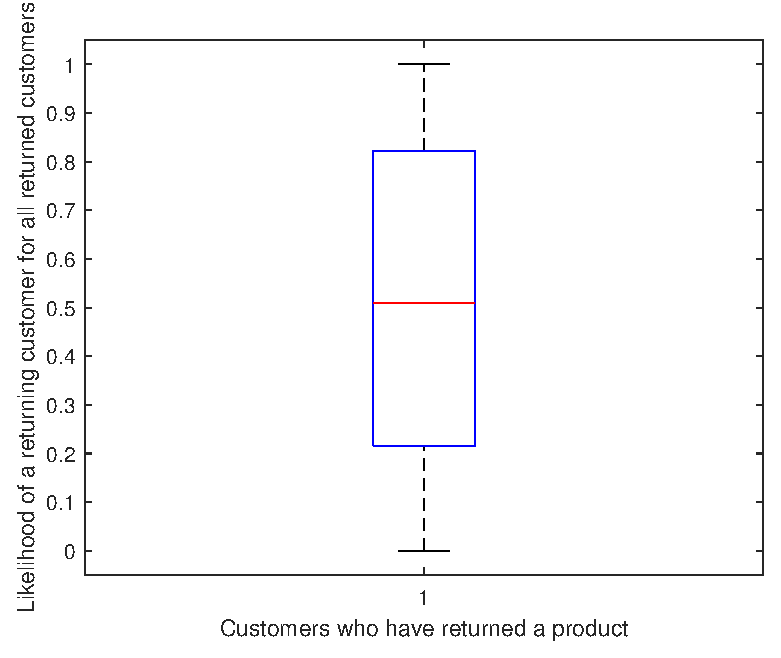
\includegraphics{boxFig}
    \caption{Box plot of likelihood}
\end{figure}
As we see from the box plot, the data is evenly spread which minimal skew, and it is centred around 0.5. This clearly shows that a customer that has returned a product is neither more or less likely to make future orders from the company. Hence we reject the hypothesis that a customer is less likely to make future orders from the company using the results from above.
The full code for question 2 can be seen in \apref{2_fullCode}.

\section{Question 3}
For this question, we want to find the top 100 customers who have purchased a product in category `C', and who have the highest weighted average of: the average product value per order in category `C', and the average rating of purchases in category `C'.

\subsection{Finding the customers who bought a product from category `C'}
Similarly to the beginning of question 2 we use \hl{readtable} to read the data into a table, and instead of filtering by \hl{Rating}, we instead filter by \hl{Product_Category} to equal `C'. We also use the same method of getting the unique customers. Altogether the code looks like:
\begin{lstlisting}[title={Reading and filtering}]
% Read file and format into table.
dataTable = readtable('purchasing_order.csv');
% Get a new subtable of dataTable, where we filter for all rows who have
% bought a product from category 'C'.
filDataTable = dataTable(dataTable.Product_Category == "C", :);
% Get the unique customer ids from the filtered table, using the first
% customer id found in case of duplicates.
[ID,index] = unique(filDataTable.Customer_ID);
uniTable = filDataTable(index, {'Customer_ID'});
\end{lstlisting}

\subsection{Choosing the weights}
Before we start to find the weighted averages for each unique customer, we need to choose the weightings for the two criteria. As we want both the average rating and average product value to be taken into account equally, then we want to choose weighting which allows either criteria to make large effects to the weighted average. We note that the product values are typically much higher than the ratings (so a typical average would take the product value more into account than the rating), so we want to keep the product values the same, while choosing a weighting for the rating which allows for it to have an similar impact on the weighted average. To do so, simply choose the weight for the product values as one, and the weight for the rating as the mean of the product values over the mean of the rating (not including the zero ratings), in the \hl{filDataTable}. The code would simply be:
\begin{lstlisting}[title={Find the weights}]
% Find weights:
valueWeight = 1;
rateWeight = mean(filDataTable.Product_Value)/ ...
             mean(filDataTable.Rating(filDataTable.Rating~=0));
\end{lstlisting}

\subsection{Find the weighted average for each unique customer}
To find the weighted average for each customer, we simply loop through each row in the \hl{uniTable} table, find its associated average value and average rating, and then the weighted average, and append each result in their respective column. When calculating the average rating, we do not take into account any ratings of zero as it could skew the overall average rating for that customer. Since we do this, then we need to include a simply check afterwards in case a particular customer has all their ratings as zero, resulting in their average rating being NaN. In this case then we just set there average rating as zero, as one of our goals is to get customers who have rated highly. The code for doing this is given as:
\begin{lstlisting}[title={Find the weighted average}]
% Loop through each customer in uniTable, and find there average product
% value, average rating and then the wieghted average.
for ind = 1:height(uniTable)
    % Get unique customer for current index.
    customer = uniTable.Customer_ID(ind);
    % Get subtable of all purchases of product 'C' by that customer.
    table = filDataTable(filDataTable.Customer_ID == customer, :);
    % Calculate the average value and rating for that customer.
    avrValue = mean(table.Product_Value);
    avrRating = mean(table.Rating(table.Rating~=0));
    % Check avrRating isn't NaN due to not having rated a product.
    if isnan(avrRating)
        avrRating = 0;
    end
    % Append the average value, rating, and then the weighted average to uniTable.
    uniTable.avrValue(ind) = avrValue;
    uniTable.avrRating(ind) = avrRating;
    uniTable.weightedAvr(ind) = (valueWeight*avrValue+rateWeight*avrRating)/ ...
                                (valueWeight+rateWeight);
end
\end{lstlisting}

\subsection{Sorting and getting results}
Now that we have the weighted average for each unique customer who has bought a product from category `C', we now need to sort the rows in descending order of there weighted average. We use the function \hl{sortrows} to sort the table according to the \hl{weightedAvr} column, and passing in the \hl{descend} parameter. After that, for convenience I assign a simple incrementing \hl{id} column from one, so that we can see position of the customer in the table. Finally we can print out our first 100 rows from our table, which correspond to the customers who we should send the coupons to. The code for this is given as (however we only will print the first five and last five entries of the top 100 customers):
\begin{lstlisting}[title={Find the weighted average}]
% Sort rows according to there weightedAvr column, from highest to lowest.
uniTable = sortrows(uniTable, 'weightedAvr', 'descend');
% Add simple increasing id for each purchase.
uniTable.id = (1:height(uniTable)).';
% Get the first and last five rows from uniTable
uniTable([1:5,96:100],:)
\end{lstlisting}
which gives an output of:
\begin{lstlisting}[title={Find the weighted average}]
ans =
  10x5 table

    Customer_ID    avrValue    avrRating    weightedAvr    id
    ___________    ________    _________    ___________    ___

    1.0143e+06        82.2          5         13.339         1
     1.012e+06        81.7          5         13.285         2
     1.015e+06        82.3          4         12.457         3
    1.0163e+06       73.35          5         12.383         4
    1.0163e+06       72.05          5         12.242         5
    1.0144e+06        49.7        4.5         9.3822        96
    1.0119e+06       45.55          5         9.3799        97
    1.0154e+06      49.667        4.5         9.3786        98
    1.0132e+06        49.6        4.5         9.3714        99
    1.0134e+06      49.467        4.5          9.357       100
\end{lstlisting}
The full code is given in \apref{3_fullCode}.

\section*{Appendix}
\begin{lstlisting}[caption={Question 1 full code},label={1_fullCode}]
%% Optimise the logreg function to find the parameters values
% Read file and format into table.
dataTable = readtable('purchasing_order.csv');
% Filter out data where rating is 0.
dataTable(dataTable.Rating == 0, :) = [];
% Get 2 arrays from the table columns of Rating and Return.
% We just pass in the Rating column from dataTable.
Rating = table2array(dataTable(:, 'Rating'));
% Note we want our array in terms of Pass (1) or fail (0), not 'Y' or 'N',
% so we do a simply boolean equality check against 'Y' for each element in
% the column. We check against the string "Y", as table2array returns an
% array of cells.
Return = table2array(dataTable(:, 'Return')) == "Y";
% Create a short function, which gets the sum of the entries, of the
% difference between the true value of the Return (p) and the logarithmic
% function, for the logarithmic parameters (a), and the Rating input (h).
logreg = @(a,h,p) sum((p-(1+exp(-a(1)*h-a(2))).^(-1)).^2);
% Find the parameters (a) which minimise the sum difference of logreg,
% given the data of Rating and Return.
a = fminsearch(@(a) logreg(a, Rating, Return), [0 0]);
a % Print the value.

%%  Make a graph, to visually see if the the model is correct.
% Create vector of 1 to 5 integers.
x = linspace(1, 5, 5)
% Create vector using regression function with found parameters, and pass
% in ratings from x.
y = (1+exp(-(x*a(1)+a(2)))).^-1
% Plot the raw data and logistic function.
plot(Rating, Return, '*', x, y)
% Add legend to graph.
lg = legend('Raw Data', 'Logistic Regression');
% Label x and y axis.
xlabel('Rating');
ylabel('Probability of return')

%% Simply checks
% Print the number of rows where the Rating column is greater than or equal
% to 2, and has a return.
height(dataTable((dataTable.Rating >= 2) & (dataTable.Return == "Y"), :))
% Get the subtable from dataTable with a rating of 1.
oneRating = dataTable(dataTable.Rating == 1, :);
% Print the percentage of those who returned the product against all the
% purchases from the oneRating table.
height(oneRating(oneRating.Return == "Y", :))/height(oneRating)
\end{lstlisting}

\begin{lstlisting}[caption={Question 2 full code},label={2_fullCode}]
% Read file and format into table.
dataTable = readtable('purchasing_order.csv');
% Get a new subtable of dataTable, where we filter for all rows who have
% returned a product.
filDataTable = dataTable(dataTable.Return == "Y", :);
% Get the unique customer ids from the filtered table, using the first
% customer id found in case of duplicate purchases.
[ID,index] = unique(filDataTable.Customer_ID);
uniTable = filDataTable(index,:);
% For each customer in uniTable, find the total sum of there bough products
% cost, before there first returned product, and after. Note we ignore any
% purchases that have been returned by the customer.
for ind = 1:height(uniTable)
    % Get associated customer id and subtable of all purchases by that
    % customer.
    customer = uniTable.Customer_ID(ind);
    table = dataTable(dataTable.Customer_ID == customer, :);
    % Remove all refunded purchases.
    table(ismember(table.Return, "Y"), :) = [];
    % Add two new columns to uniTable, for there prepurchases and
    % postpurchases.
    uniTable.prePurchases(ind) = sum(table.Product_Value( ...
                    uniTable.Date(uniTable.Customer_ID == customer) > table.Date));
    uniTable.postPurchases(ind) = sum(table.Product_Value(...
                    uniTable.Date(uniTable.Customer_ID == customer) < table.Date));
end
% For each customer in uniTable find out there likelihood that they will
% return, given by postPurchases/(prePurchases+postPurchases)%.
uniTable.likelihood = uniTable.postPurchases.* ...
                      (uniTable.prePurchases+uniTable.postPurchases).^-1;
% Find the mean and median of the likelihood column in table uniTable.
likeMean = mean(uniTable.likelihood)
likeMedian = median(uniTable.likelihood)
% Draw boxplot using likelihood column data from uniTable.
boxplot(uniTable.likelihood);
% Label the x and y axis.
xlabel("Customers who have returned a product");
ylabel("Likelihood of a returning customer for all returned customers");
% Save box plot as file.
print -depsc boxFig;
\end{lstlisting}

\begin{lstlisting}[caption={Question 3 full code},label={3_fullCode}]
% Read file and format into table.
dataTable = readtable('purchasing_order.csv');
% Get a new subtable of dataTable, where we filter for all rows who have
% bought a product from category 'C'.
filDataTable = dataTable(dataTable.Product_Category == "C", :);
% Get the unique customer ids from the filtered table, using the first
% customer id found in case of duplicates.
[ID,index] = unique(filDataTable.Customer_ID);
uniTable = filDataTable(index, {'Customer_ID'});
% Find weights:
valueWeight = 1;
rateWeight = mean(filDataTable.Product_Value)/ ...
             mean(filDataTable.Rating(filDataTable.Rating~=0));
% Loop through each customer in uniTable, and find there average product
% value, average rating and then the wieghted average.
for ind = 1:height(uniTable)
    % Get unique customer for current index.
    customer = uniTable.Customer_ID(ind);
    % Get subtable of all purchases of product 'C' by that customer.
    table = filDataTable(filDataTable.Customer_ID == customer, :);
    % Calculate the average value and rating for that customer.
    avrValue = mean(table.Product_Value);
    avrRating = mean(table.Rating(table.Rating~=0));
    % Check avrRating isn't NaN due to not having rated a product.
    if isnan(avrRating)
        avrRating = 0;
    end
    % Append the average value, rating, and then the weighted average to uniTable.
    uniTable.avrValue(ind) = avrValue;
    uniTable.avrRating(ind) = avrRating;
    uniTable.weightedAvr(ind) = (valueWeight*avrValue+rateWeight*avrRating)/ ...
                                (valueWeight+rateWeight);
end
% Sort rows according to there weightedAvr column, from highest to lowest.
uniTable = sortrows(uniTable, 'weightedAvr', 'descend');
% Add simple increasing id for each purchase.
uniTable.id = (1:height(uniTable)).';
% Get the first and last five rows from uniTable
uniTable([1:5,96:100],:)
\end{lstlisting}


\end{document}

% Replace columns names with \hl
% Go through quest 3.2 and beyond
